\documentclass[professionalfont]{beamer}

\usepackage{graphicx}
\usepackage{newtxtext,newtxmath}
\usepackage[backend=bibtex]{biblatex} 
\addbibresource{ref.bib}
\renewcommand*{\bibfont}{\scriptsize}

\usetheme{default}
\usecolortheme{seagull}

\setbeamertemplate{navigation symbols}{}
\setbeamertemplate{itemize item}{\textbullet} 
\setbeamertemplate{bibliography item}[text]
\setbeamertemplate{title page}{
    \begin{center}
        {\textcolor{blue}{\textbf{\fontsize{13}{14}\selectfont
        Language Models are Unsupervised Multitask Learners}}} \\[1.5cm]
        
        {\fontsize{9}{14}\selectfont Alec Radford, et al \\[0.3cm]
        OpenAI \\[0.3cm]
        2019}
    \end{center}
}
% ------------------ Title ------------------

\begin{document}
\frame{\titlepage}

\begin{frame}
\begin{center}
    { \textbf{\textcolor{blue}{ {\fontsize{12}{14}\selectfont Abstract} }} }
\end{center}
\\[0.5cm]

{\fontsize{10}{14}\selectfont 
\begin{itemize}
    \item NLP Tasks were approached with supervised learning
    
    - Labeling and fine-tuning for a specific task
    
    - Not enough generalization

    \\[0.5cm]

    \item We suggest unsupervised multitask, achieved by

    - Large model GPT-2 (1.5B Parameters)

    - Huge dataset of millions of webpages called WebText
\end{itemize}
}

\end{frame}
% ------------------ Slide 1 ------------------

\begin{frame}
\begin{center}
    { \textbf{\textcolor{blue}{ {\fontsize{12}{14}\selectfont Introduction} }} }
\end{center}
\\[0.5cm]

{\fontsize{10}{14}\selectfont 
\begin{itemize}
    \item Problem of ``Narrow expert"
    
    - Single task training on single domain dataset
    
    - Sensitive to slight changes in the data distribution

    - Poor performance on GLUE, decaNLP

    \\[0.5cm]

    \item We try to make ``Competent generalists"

    - Unsupervised pre-training

    - Zero-shot setting (No fine-tuning)
\end{itemize}
}

\end{frame}
% ------------------ Slide 2 ------------------

\begin{frame}
\begin{refsection}

\begin{center}
    { \textbf{\textcolor{blue}{ {\fontsize{12}{14}\selectfont Approach } }} }
\end{center}
\\[0.5cm]

{\fontsize{10}{14}\selectfont 
\begin{itemize}
    \item Traditional Language models

    - Estimate conditional distribution \( p(output|input) \)
    
    \\[0.5cm]
    
    \item Multitask and meta-learning settings

    - Estimate conditional distribution \( p(output|input, task) \)

    - Find triplet \( (input, output, task) \) in natural language sentence
    
    - It is achieved by MQAN \cite{MQAN}

    - We expect sufficient data and model size can perform it
\end{itemize}
}

\vspace{0.5cm}
\hrule
\printbibliography
\end{refsection} 
\end{frame}
% ------------------ Slide 3 ------------------

\begin{frame}
\begin{center}
    { \textbf{\textcolor{blue}{ {\fontsize{12}{14}\selectfont Training dataset} }} }
\end{center}
\\[0.5cm]

{\fontsize{10}{14}\selectfont 
\begin{itemize}
    \item Prior works used single domain dataset
    
    - News articles, Wikipedia, Fiction books

    \\[0.5cm]

    \item We used WebText, containing 45 million links

    - We scraped links from Reddit, which received at least 3 karma

    - De-duplication and some heuristic based cleaning

    - 8 million documents for a total of 40 GB of text
\end{itemize}
}

\end{frame}
% ------------------ Slide 4 ------------------

\begin{frame}
\begin{center}
    { \textbf{\textcolor{blue}{ {\fontsize{12}{14}\selectfont Input Representation} }} }
\end{center}
\\[0.5cm]

{\fontsize{10}{14}\selectfont 
\begin{itemize}
    \item Word-level Models
    
    - Preprocessing is needed

    - Lowercasing, Tokenization, Out-of-vocabulary tokens

    \\[0.5cm]

    \item Byte-level Models

    - Treating text as UTF-8 bytes without preprocessing

    - Low performance on large scale datasets

    - 8 million documents for a total of 40 GB of text
\end{itemize}
}

\end{frame}
% ------------------ Slide 5 ------------------
\begin{frame}
\begin{refsection}

\begin{center}
    { \textbf{\textcolor{blue}{ {\fontsize{12}{14}\selectfont Input Representation} }} }
\end{center}
\\[0.5cm]

{\fontsize{10}{14}\selectfont 
\begin{itemize}
    \item Byte Pair Encoding (BPE) \cite{BPE}

    - Treating frequent pairs as a token

    - ex) preprocess \( \rightarrow \) `pre', `process'

    \\[0.3cm]

    - If character categories are different, they are divided

    - Categories include letters, numbers, punctuation

    - ex) fair-play \( \rightarrow \) `fair', `play'

    \\[0.5cm]

    \item Byte-level BPE (BBPE)

    - Despite its name, BPE operates on Unicode code points

    - We changed it to byte-level instead of Unicode symbols
\end{itemize}
}

\vspace{0.3cm}
\hrule
\printbibliography

\end{refsection}
\end{frame}
% ------------------ Slide 6 ------------------

\begin{frame}
\begin{center}
    { \textbf{\textcolor{blue}{ {\fontsize{12}{14}\selectfont Model} }} }
\end{center}
\\[0.3cm]
\begin{center}
    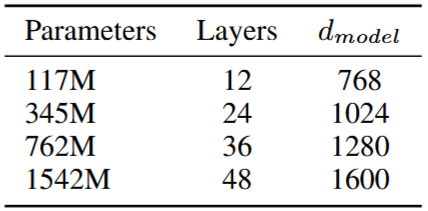
\includegraphics[width=0.5\textwidth]{table2.png}
\end{center}

{\fontsize{10}{14}\selectfont 
\begin{itemize}
    \item The 4 models largely follow the details of the OpenAI GPT

    \item Few modifications of layer normalizations

    - It moved to the input of each sub-block

    - Additional normalization after the final self attention

    \item A modified initialization

    - Scaled weights of residual layers by \( \frac{1}{\sqrt{N}} \)

    - \( N \) is the number of residual layers
\end{itemize}
}

\end{frame}
% ------------------ Slide 7 ------------------

\begin{frame}
\begin{center}
    { \textbf{\textcolor{blue}{ {\fontsize{12}{14}\selectfont Experiment} }} }
\end{center}
\\[0.3cm]
\begin{center}
    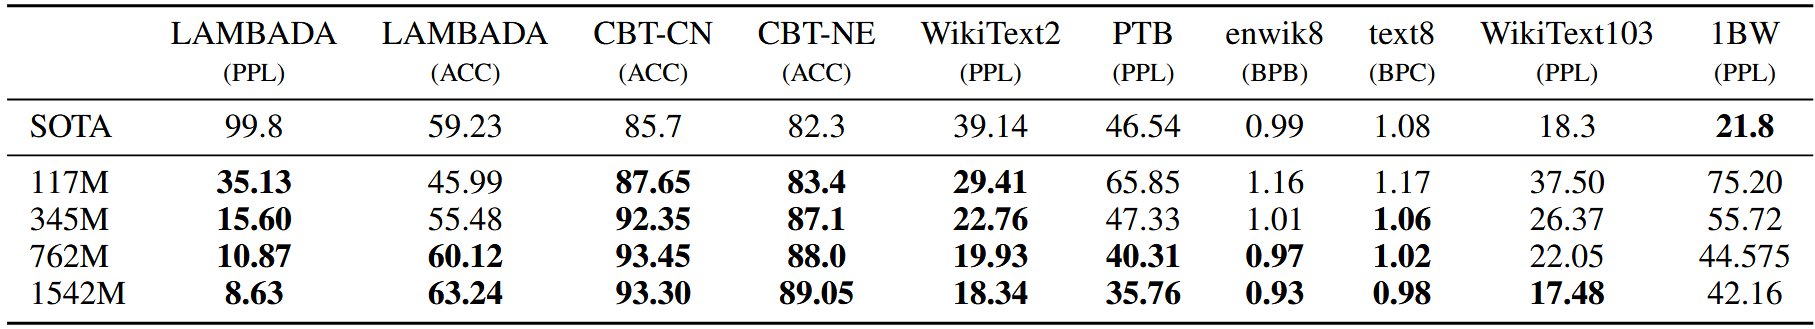
\includegraphics[width=1.0\textwidth]{table3.png}
\end{center}

{\fontsize{10}{14}\selectfont 
\begin{itemize}
    \item Accuracy (ACC)
    
    - Correctness of word prediction

    \item Perplexity (PPL)
    
    - How "surprised" the model is by the data

    \item Bits per Byte (BPB)
    
    - It measures the compression efficiency of a model

    \item Bits per Character (BPC)
    
    - It measures the compression efficiency of a model

\end{itemize}
}

\end{frame}
% ------------------ Slide 8 ------------------

\begin{frame}
\begin{refsection}

\begin{center}
    { \textbf{\textcolor{blue}{ {\fontsize{12}{14}\selectfont Experiment} }} }
\end{center}
\\[0.3cm]
\begin{center}
    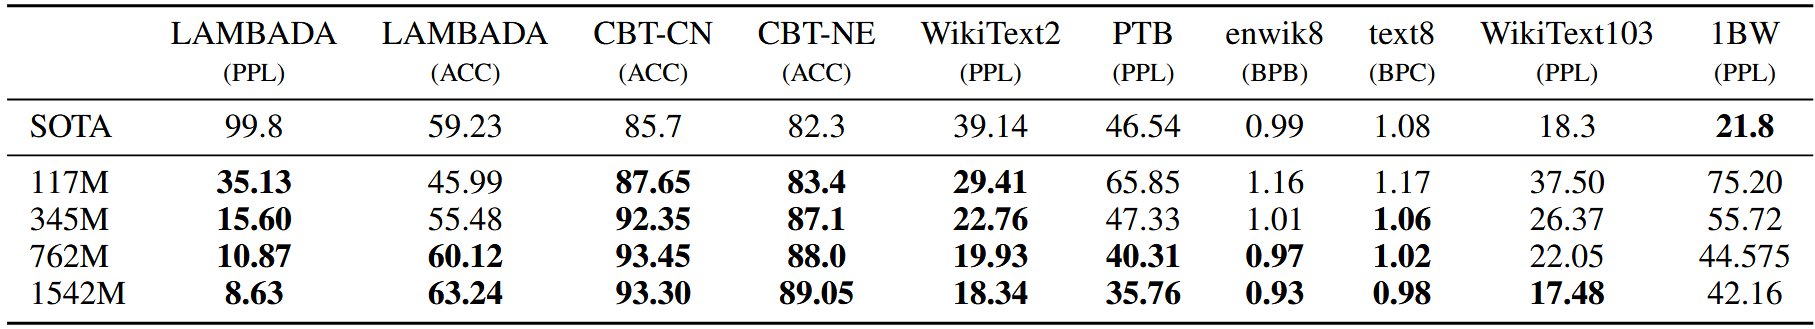
\includegraphics[width=1.0\textwidth]{table3.png}
\end{center}

{\fontsize{10}{14}\selectfont 
\begin{itemize}
    \item SOTA on many datasets (Not most of datasets)
    
    - Large improvements on small datasets (PTB, WikiText2)

    - Large improvements on long-term dependency (LAMBADA, CBT)

    \item Worse performance on 1BW \cite{1BW}
    
    - It is the biggest dataset

    - Sentence level shuffling to remove long-range structure

\end{itemize}
}

\vspace{0.3cm}
\hrule
\printbibliography 

\end{refsection}
\end{frame}
% ------------------ Slide 9 ------------------

\begin{frame}

\begin{center}
    { \textbf{\textcolor{blue}{ {\fontsize{12}{14}\selectfont Children’s Book Test} }} }
\end{center}
\\[0.3cm]
\begin{center}
    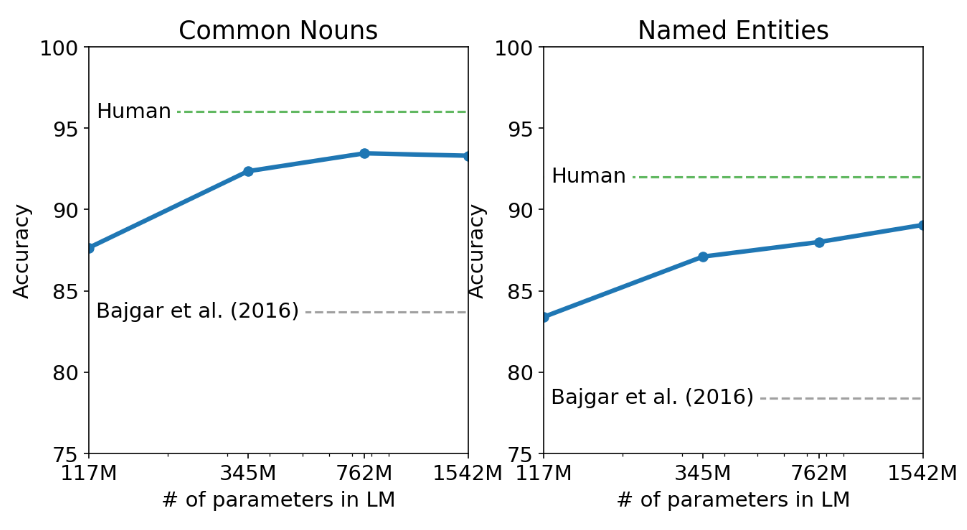
\includegraphics[width=0.7\textwidth]{figure2.png}
\end{center}

{\fontsize{10}{14}\selectfont 
\begin{itemize}
    \item Predicting missing words in the sentence

    \item Common Nouns (CN)
    
    - Dog, Cat, Window, ...

    \item Name Entities (NE)
    
    - Alice, Bob, Jack, ...

\end{itemize}
}

\end{frame}
% ------------------ Slide 10 ------------------

\begin{frame}

\begin{center}
    { \textbf{\textcolor{blue}{ {\fontsize{12}{14}\selectfont LAMBADA} }} }
\end{center}
\\[0.3cm]

{\fontsize{10}{14}\selectfont 
\begin{itemize}
    \item Test ability to handle long-range dependencies

    - Prediction of the final word in a sentence

    \\[0.3cm]

    \item Stop-Word filtering

    - The predicted word must logically end the sentence
    
    - GPT-2 was not leveraging the constraint

    - By excluding words like `and', `the', GPT-2 achieved SOTA

\end{itemize}
}

\end{frame}
% ------------------ Slide 11 ------------------

\begin{frame}

\begin{center}
    { \textbf{\textcolor{blue}{ {\fontsize{12}{14}\selectfont Winograd Schema Challenge} }} }
\end{center}
\\[0.3cm]
\begin{center}
    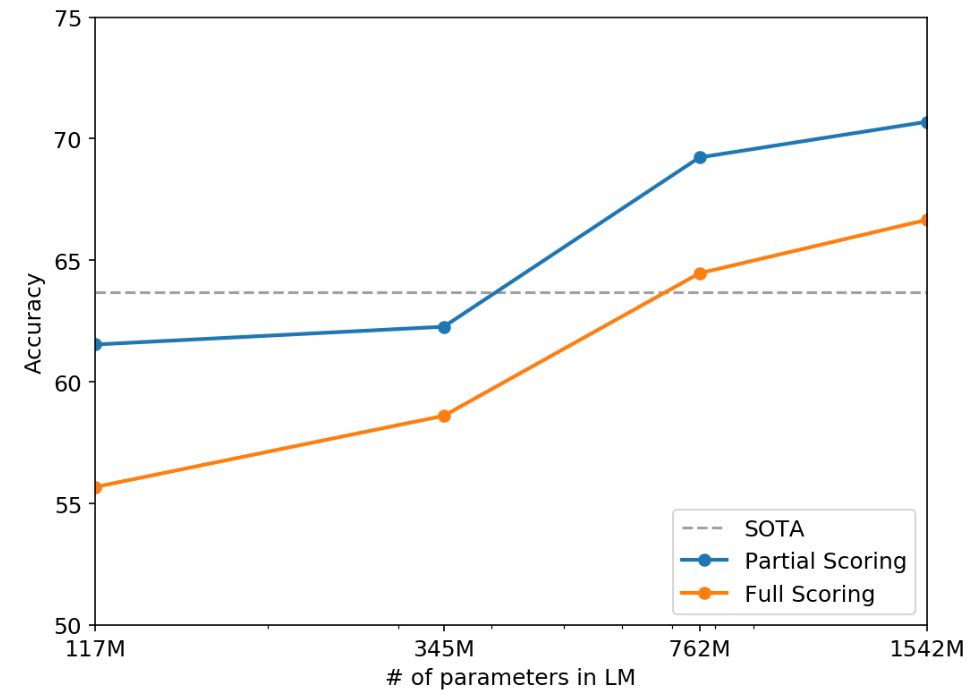
\includegraphics[width=0.6\textwidth]{figure3.png}
\end{center}

{\fontsize{10}{14}\selectfont 
\begin{itemize}
    \item Commonsense reasoning by resolving textual ambiguities.
    
    - ``The trophy doesn't fit in the suitcase because it is too small."
    
    - What does `it' refer to? (Answer: ``the suitcase.")

\end{itemize}
}

\end{frame}
% ------------------ Slide 12 ------------------

\begin{frame}
\begin{refsection}

\begin{center}
    { \textbf{\textcolor{blue}{ {\fontsize{12}{14}\selectfont Reading Comprehension} }} }
\end{center}
\\[0.3cm]

{\fontsize{10}{14}\selectfont 
\begin{itemize}
    \item Conversation Question Answering dataset (CoQA) \cite{coqa}
    
    - Dialogues between a question asker and a question answerer
    
    - Answer questions that depend on conversation history

    \\[0.3cm]

    \item Achieved 55 F1 Score

    - Supervised SOTA is nearing the 89 F1

    - GPT-2 used simple retrieval based heuristics

\end{itemize}
}

\vspace{0.3cm}
\hrule
\printbibliography 

\end{refsection}
\end{frame}
% ------------------ Slide 13 ------------------

\begin{frame}

\begin{center}
    { \textbf{\textcolor{blue}{ {\fontsize{12}{14}\selectfont Summarization} }} }
\end{center}
\\[0.3cm]
\begin{center}
    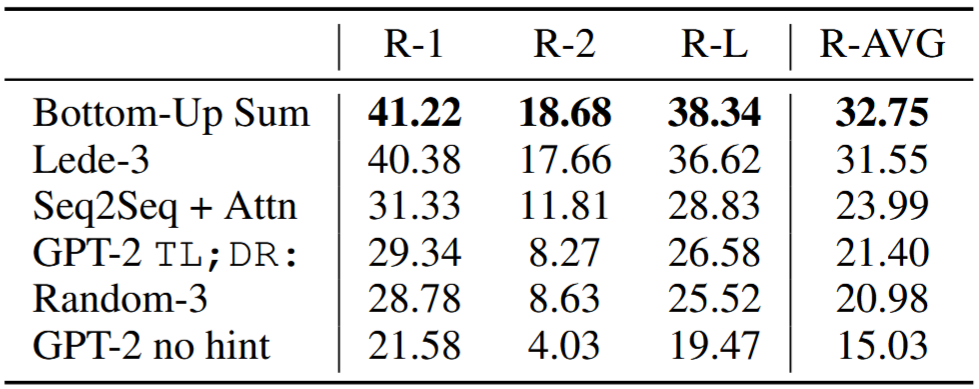
\includegraphics[width=0.6\textwidth]{table4.png}
\end{center}

{\fontsize{10}{14}\selectfont 
\begin{itemize}
    \item CNN and Daily Mail dataset summarization
    
    - The text ``TL;DR:" is appended as a hint for the task
    
    - ROUGE 1,2,L metrics (overlap with reference summary)

    \item Poor performance
    
    - TL;DR: played important role for task recognition
\end{itemize}
}

\end{frame}
% ------------------ Slide 14 ------------------

\begin{frame}

\begin{center}
    { \textbf{\textcolor{blue}{ {\fontsize{12}{14}\selectfont Translation} }} }
\end{center}
\\[0.3cm]

{\fontsize{10}{14}\selectfont 
\begin{itemize}
    \item BLEU (Bilingual Evaluation Understudy)

    - Precision about matching n-grams

    - Brevity penalty for overly short translations

    \\[0.3cm]

    \item WMT-14 Dataset (English-French)
    
    - English to French: BLEU score 5
    
    - French to English: BLEU score 11.5

    \\[0.3cm]

    \item Poor performance

    - French data was not enough in WebText

\end{itemize}
}

\end{frame}
% ------------------ Slide 15 ------------------

\begin{frame}
\begin{refsection}

\begin{center}
    { \textbf{\textcolor{blue}{ {\fontsize{12}{14}\selectfont Question Answering} }} }
\end{center}
\\[0.3cm]

{\fontsize{10}{14}\selectfont 
\begin{itemize}
    \item Natural Questions dataset \cite{naturalquestions}
    
    - ``Who is the president of the U.S.?"

    \\[0.3cm]

    \item GPT-2 Performance

    - 4.1\% accuracy when evaluated by exact match metric

    - Five times better than the smallest model

    - Still much worse than supervised systems
\end{itemize}
}

\vspace{0.3cm}
\hrule
\printbibliography

\end{refsection}
\end{frame}
% ------------------ Slide 16 ------------------

\begin{frame}

\begin{center}
    { \textbf{\textcolor{blue}{ {\fontsize{12}{14}\selectfont Generalization vs Memorization} }} }
\end{center}
\\[0.3cm]

\begin{center}
    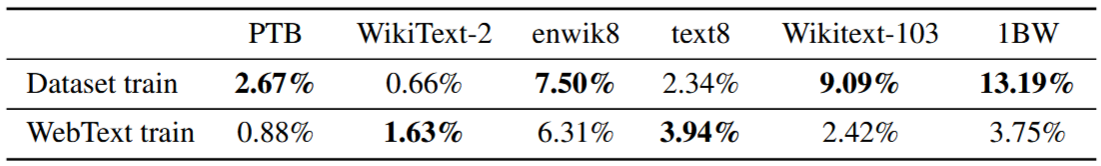
\includegraphics[width=1.0\textwidth]{table6.png}
\end{center}

{\fontsize{10}{14}\selectfont 
\begin{itemize}
    \item There may be overlap between train-test set
    
    - Bloom filters containing 8-grams

    \\[0.3cm]

    \item Overall Overlap Analysis

    - Overlap provides a small but consistent performance benefit

    - Overlap is not significantly larger than the train-test overlap

    \\[0.3cm]

    \item Testing for Memorization

    - Performance improves as model size increases

    - It indicates underfitting rather than over-memorization
\end{itemize}
}

\end{frame}
% ------------------ Slide 17 ------------------

\begin{frame}

\begin{center}
    { \textbf{\textcolor{blue}{ {\fontsize{12}{14}\selectfont Conclusion} }} }
\end{center}
\\[0.3cm]

{\fontsize{10}{14}\selectfont 
\begin{itemize}
    \item Unsupervised Task Learning

    - Performs well with sufficiently large and diverse dataset
    
    - Possibility of learning without fine-tuning

    \\[0.3cm]

    \item Limitation

    - Far from practically usable for most tasks

    - GPT-2 still struggles with structured reasoning
\end{itemize}
}

\end{frame}
% ------------------ Slide 18 ------------------
\end{document}
